\subsection{Juegos similares}

\subsubsection{Ultimate Chicken Horse}\label{subsubsec:UCH}

\emph{Ultimate Chicken Horse}, desarrollado y publicado por \emph{Clever
Endeavour Games} en el 2016, es un videojuego festivo de plataformas en el que
el jugador debe hacerse de trampas y obstáculos para colocarlas en el nivel y
así evitar que los compañeros de juego consigan llegar a la meta. Sin embargo,
el propio jugador no es inmune a sus trampas y, por tanto, debe evitar caer
también en ellas. El juego está disponible para PC, Nintendo Switch, XBOX One y
PS4 y su modelo de negocio es Buy-to-Play con DLCs.

La similitud que tiene el producto con este juego recae en el hecho de que ambos
son de los géneros \emph{festivo} y \emph{plataformas} y se fomenta la
competición entre jugadores. En efecto, éste ha podido mostrar la viabilidad que
tiene un juego de plataformas competitivo.

La página oficial es:
\url{https://www.cleverendeavourgames.com/ultimate-chicken-horse/}

\textbf{Capturas:}

\begin{figure}[H]
    \centering
    \begin{minipage}{0.43\textwidth}
        \centering
        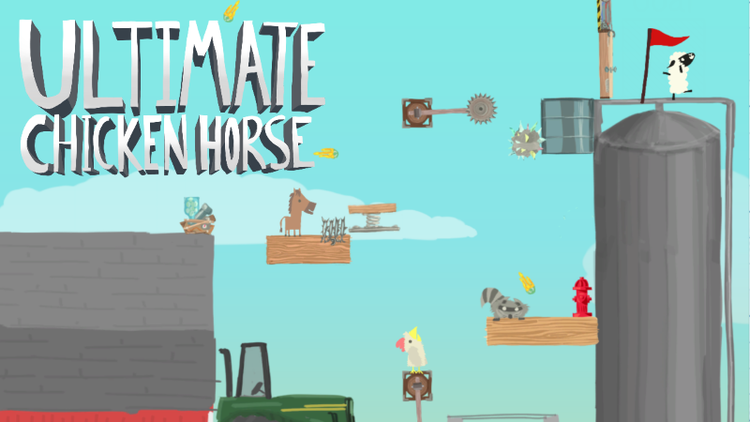
\includegraphics[width=1.0\textwidth]{Cuerpo/4/UCH1.png} %
        \subcaption{Pantalla principal del juego}
        \label{UCH-Inicio}
    \end{minipage}\hfill
    \begin{minipage}{0.43\textwidth}
        \centering
        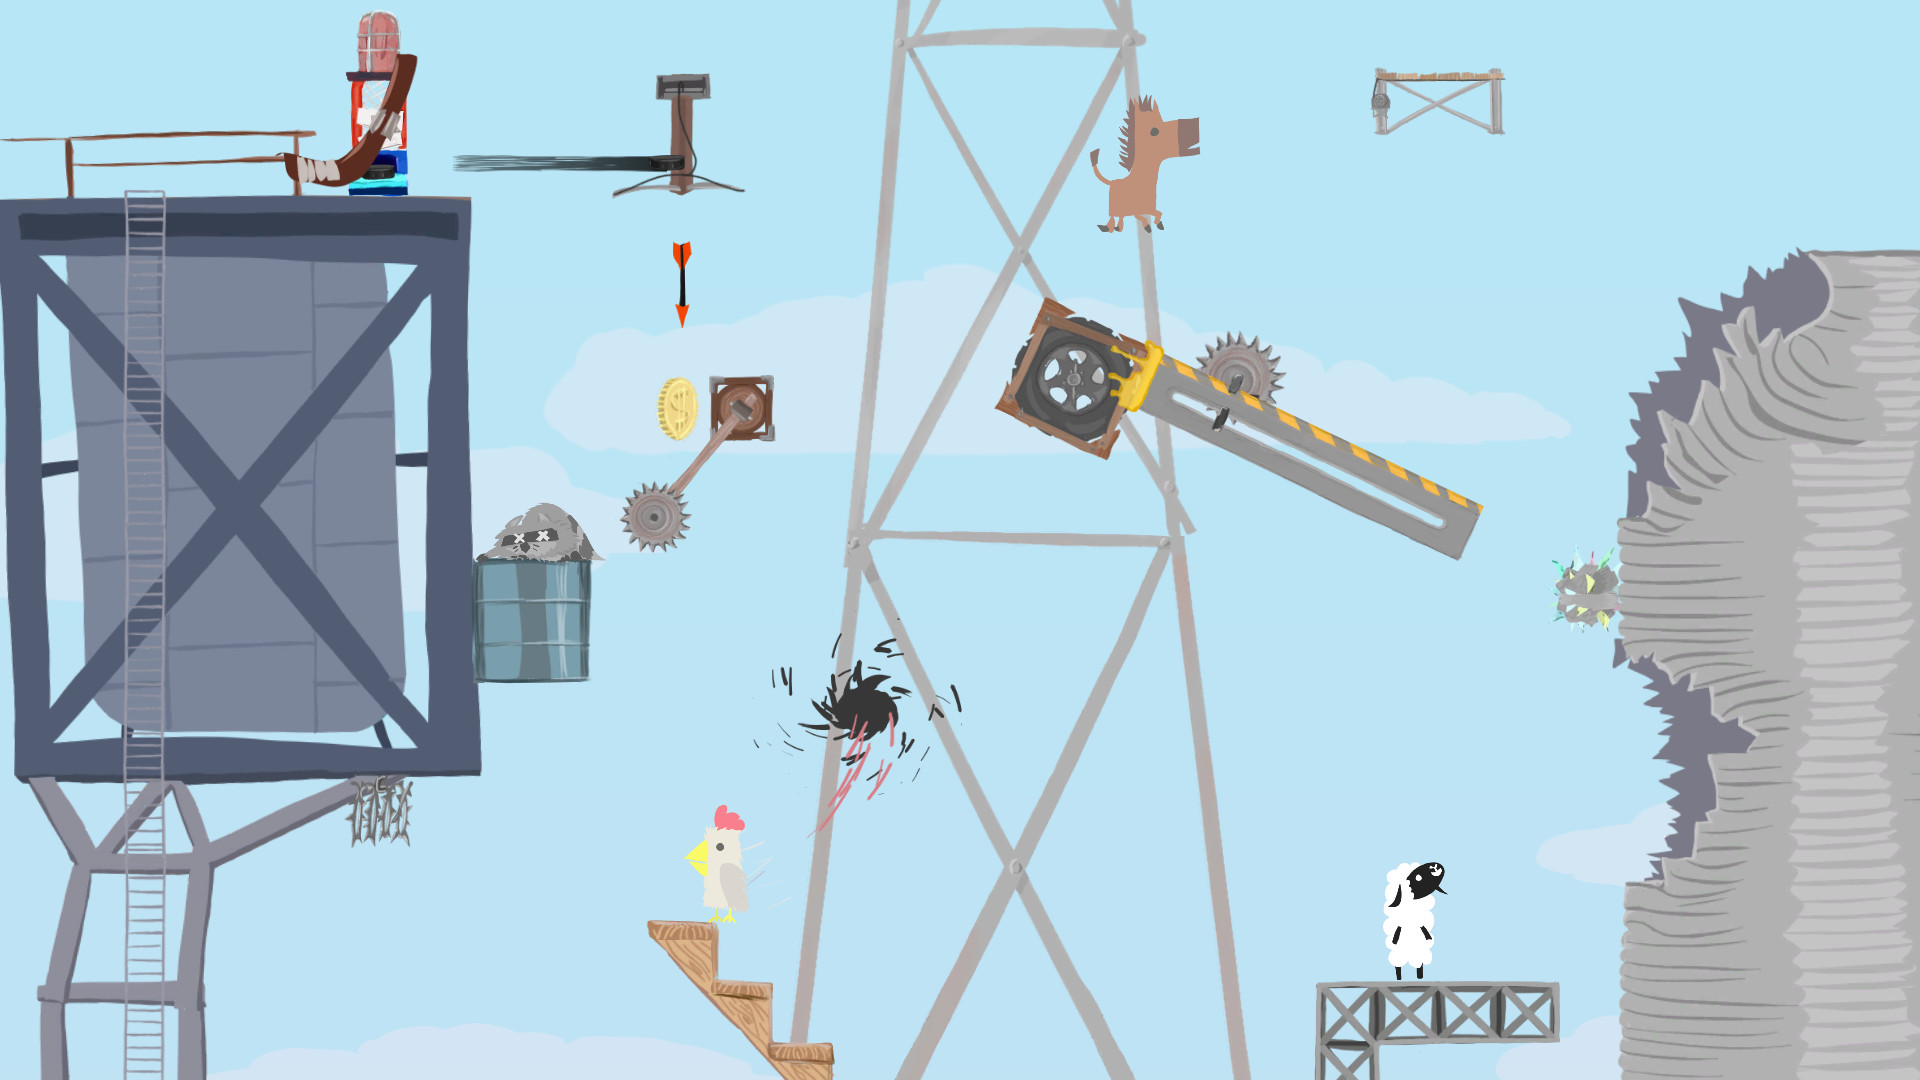
\includegraphics[width=1.0\textwidth]{Cuerpo/4/UCH2.jpg} %
        \subcaption{Algunos jugadores (animales) y obstáculos}
        \label{UCH-Jugadores}
    \end{minipage}
    \centering
    \begin{minipage}{0.43\textwidth}
        \centering
        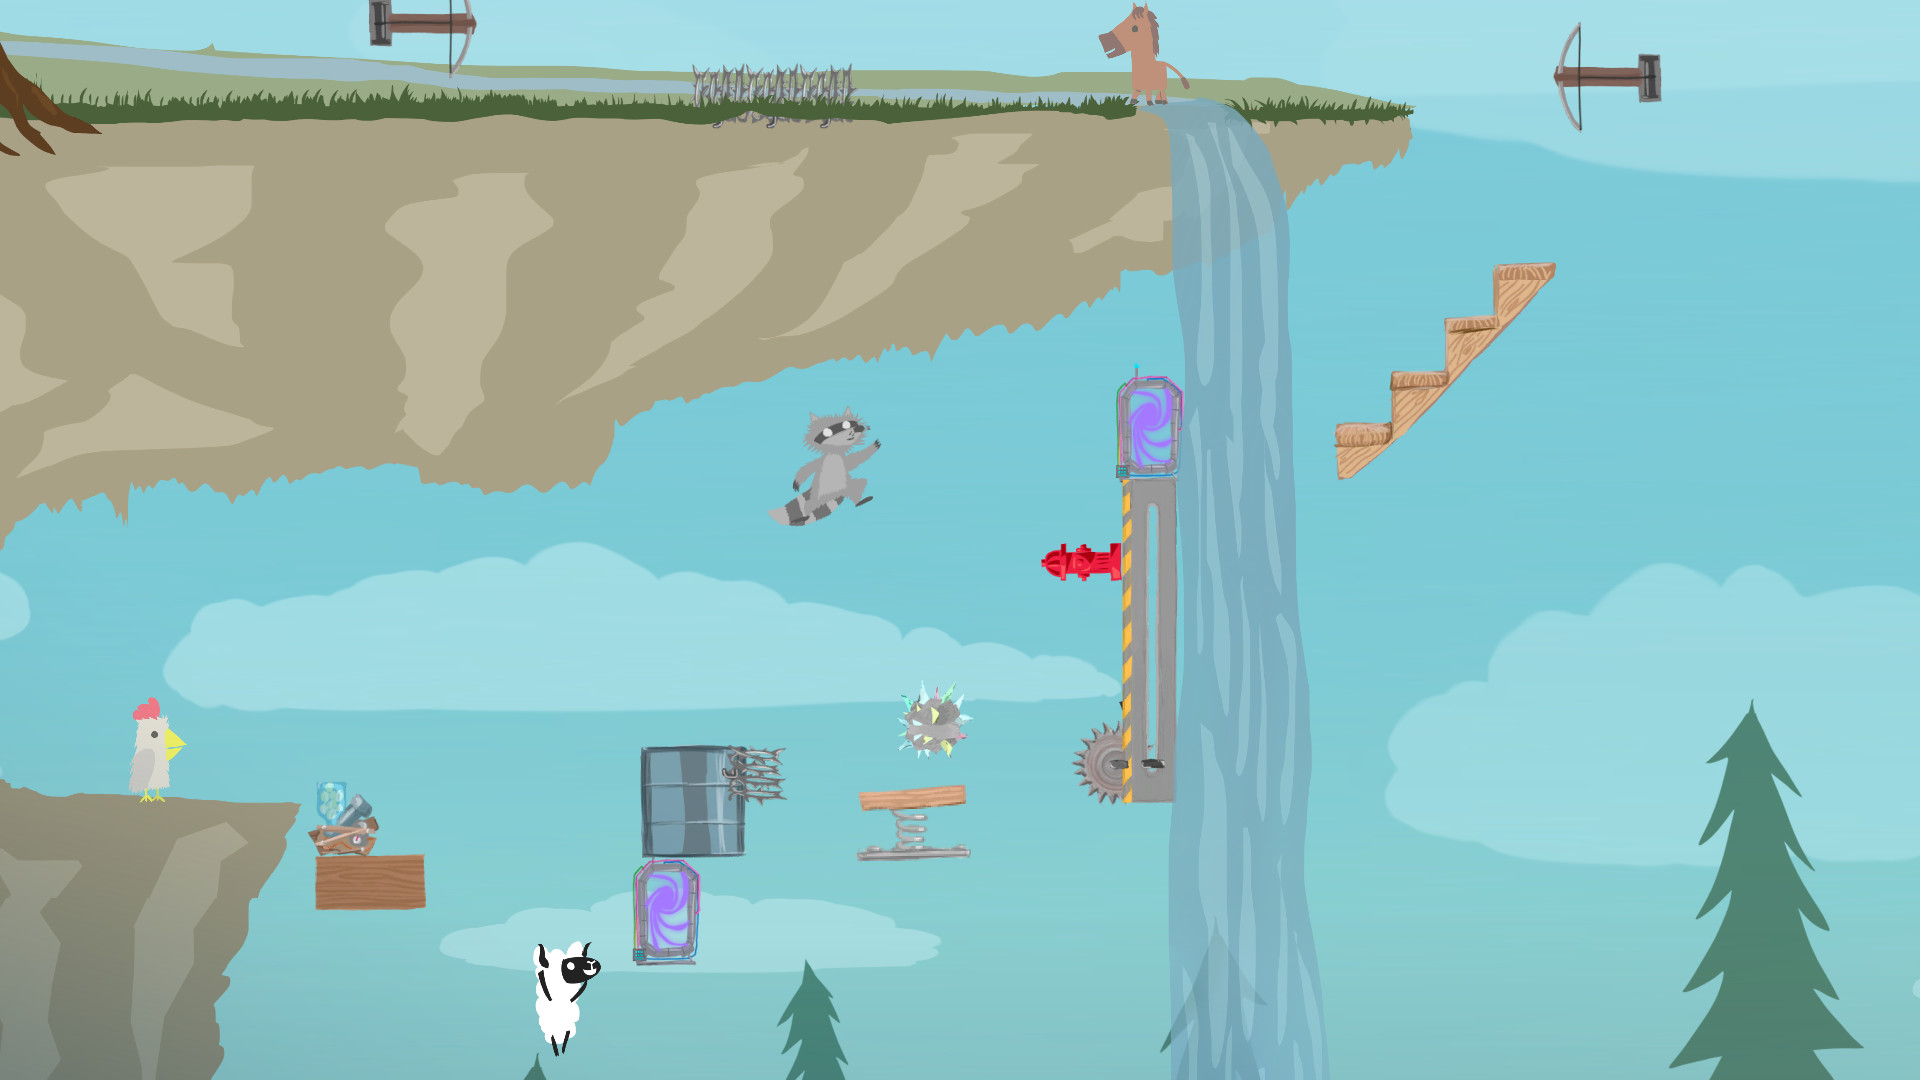
\includegraphics[width=1.0\textwidth]{Cuerpo/4/UCH3.jpg} %
        \subcaption{Un jugador cayendo hacia al vacío y otro saltando}
        \label{UCH-Muerte}
    \end{minipage}
    \caption{Capturas de Ultimate Chicken Horse}
\end{figure}

\textbf{Aspectos positivos}
\begin{itemize}
    \item Multijugador online y local hasta 4 jugadores.
    \item Dinámica de juego única que fomenta la competición.
    \item Complejo si se desea usar estrategia, simple si no.
    \item Constructor de niveles intuitivo.
    \item Distintos modos de juego.
    \item Múltiples niveles y objetos a descubrir.
\end{itemize}

\textbf{Aspectos negativos}
\begin{itemize}
    \item A pesar de ser un juego festivo, existen segmentos en los que hay que
    esperar a que todos los jugadores estén listos y esto tiende a ser lento.
    \item Los controles a veces pueden llegar a tener problemas de respuesta.
    \item Los juegos pueden hacerse largos, lo cual no es recomendable para un
    juego festivo.
\end{itemize}


\subsubsection{MicroMages} \emph{MicroMages}, desarrollado y publicado por
\emph{MorphCat Games} en el 2019, es un juego de plataformas actualmente
disponible para PC y NES. El objetivo del juego es conseguir llegar hasta la
cima de una torre infestada por monstruos y trampas, ya sea solo o jugando con
otros compañeros magos. La característica principal del juego es que ha sido
desarrollado recientemente con una restricción de memoria de 40KB, siendo además
un homenaje al género de plataformas de la NES y teniendo un modelo de negocio
Buy-to-Play.

La similitud que tiene el producto a desarrolllar con este juego recae en el
hecho de que ambos se ubican en una torre llena de monstruos y trampas. En
efecto, este videojuego ha sido una inspiración directa para la temática y
ambientación de \emph{\izenburua}.

La página oficial es:
\url{http://morphcat.de/micromages/}

\textbf{Capturas}

\begin{figure}[H]
    \centering
    \begin{minipage}{0.43\textwidth}
        \centering
        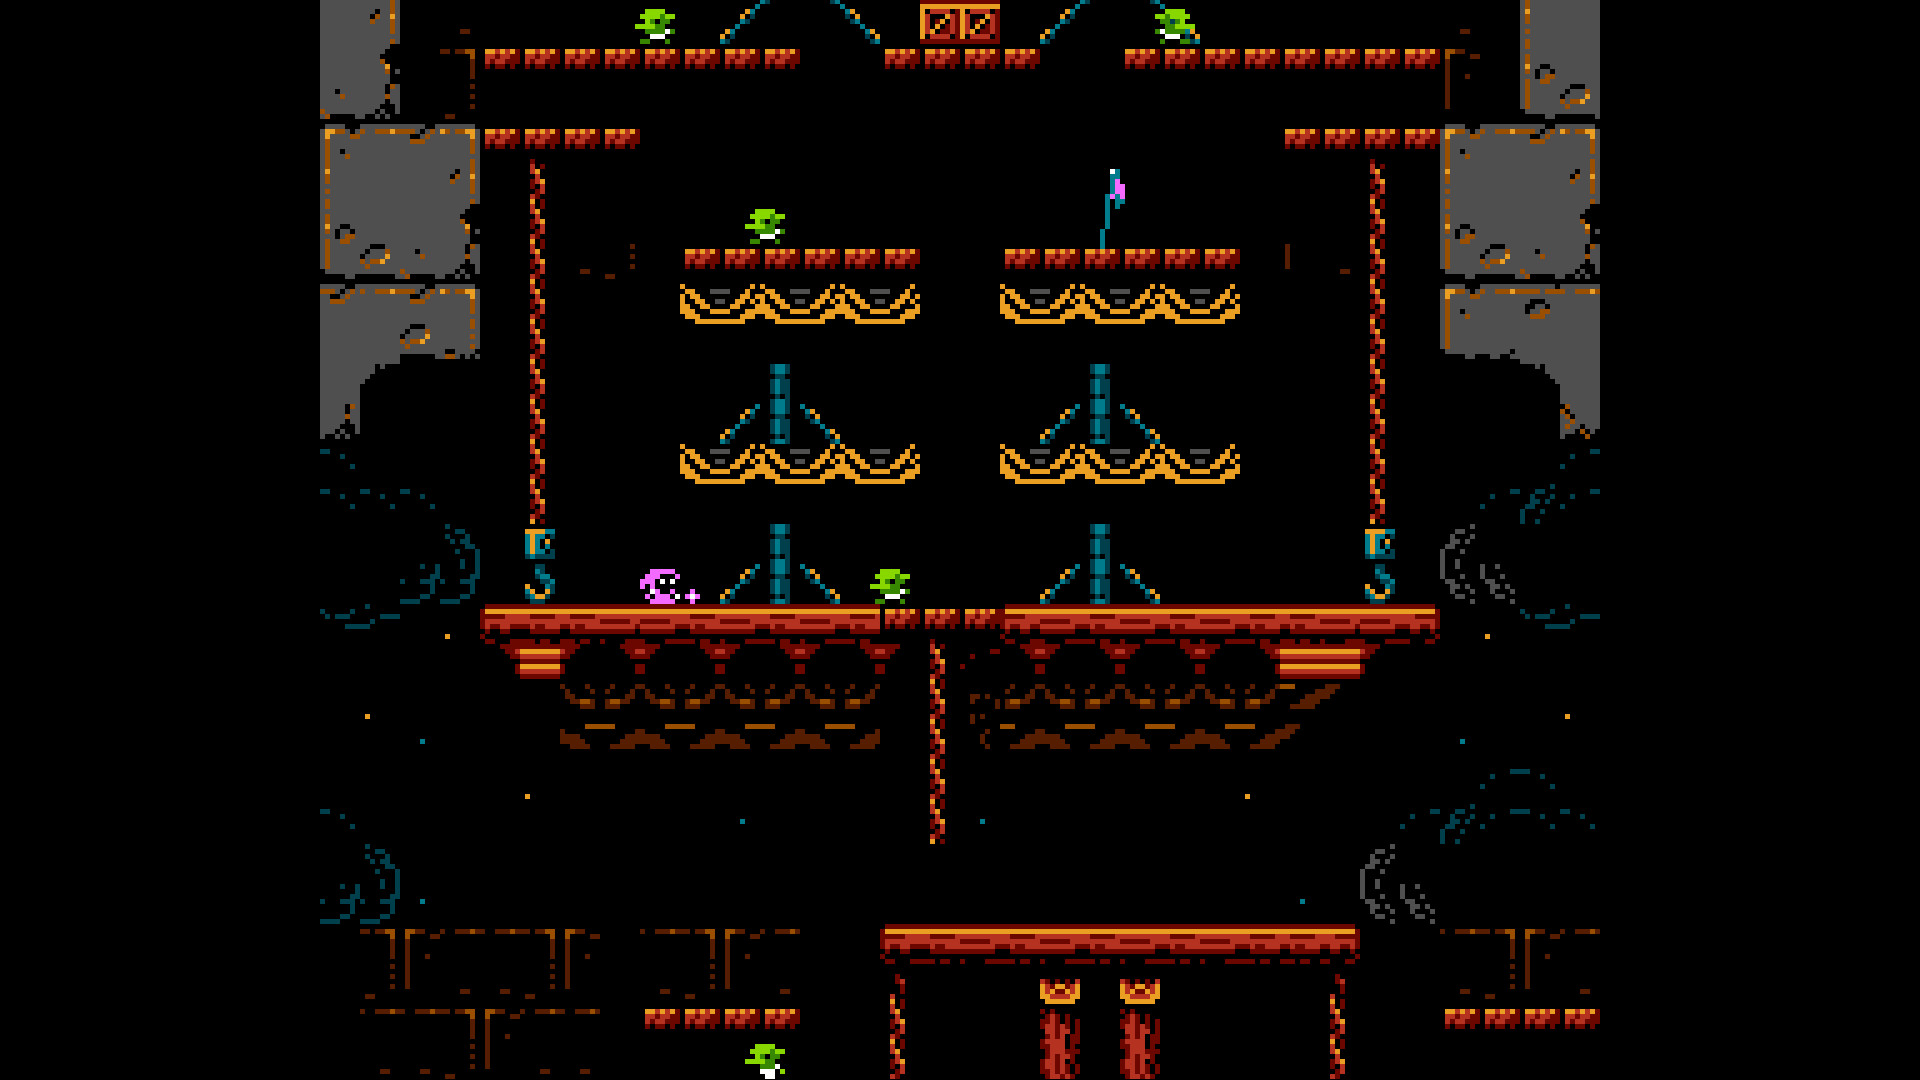
\includegraphics[width=1.0\textwidth]{Cuerpo/4/MM1.jpg} %
        \subcaption{Un nivel del juego con un jugador}
        \label{UCH-Nivel}
    \end{minipage}\hfill
    \begin{minipage}{0.43\textwidth}
        \centering
        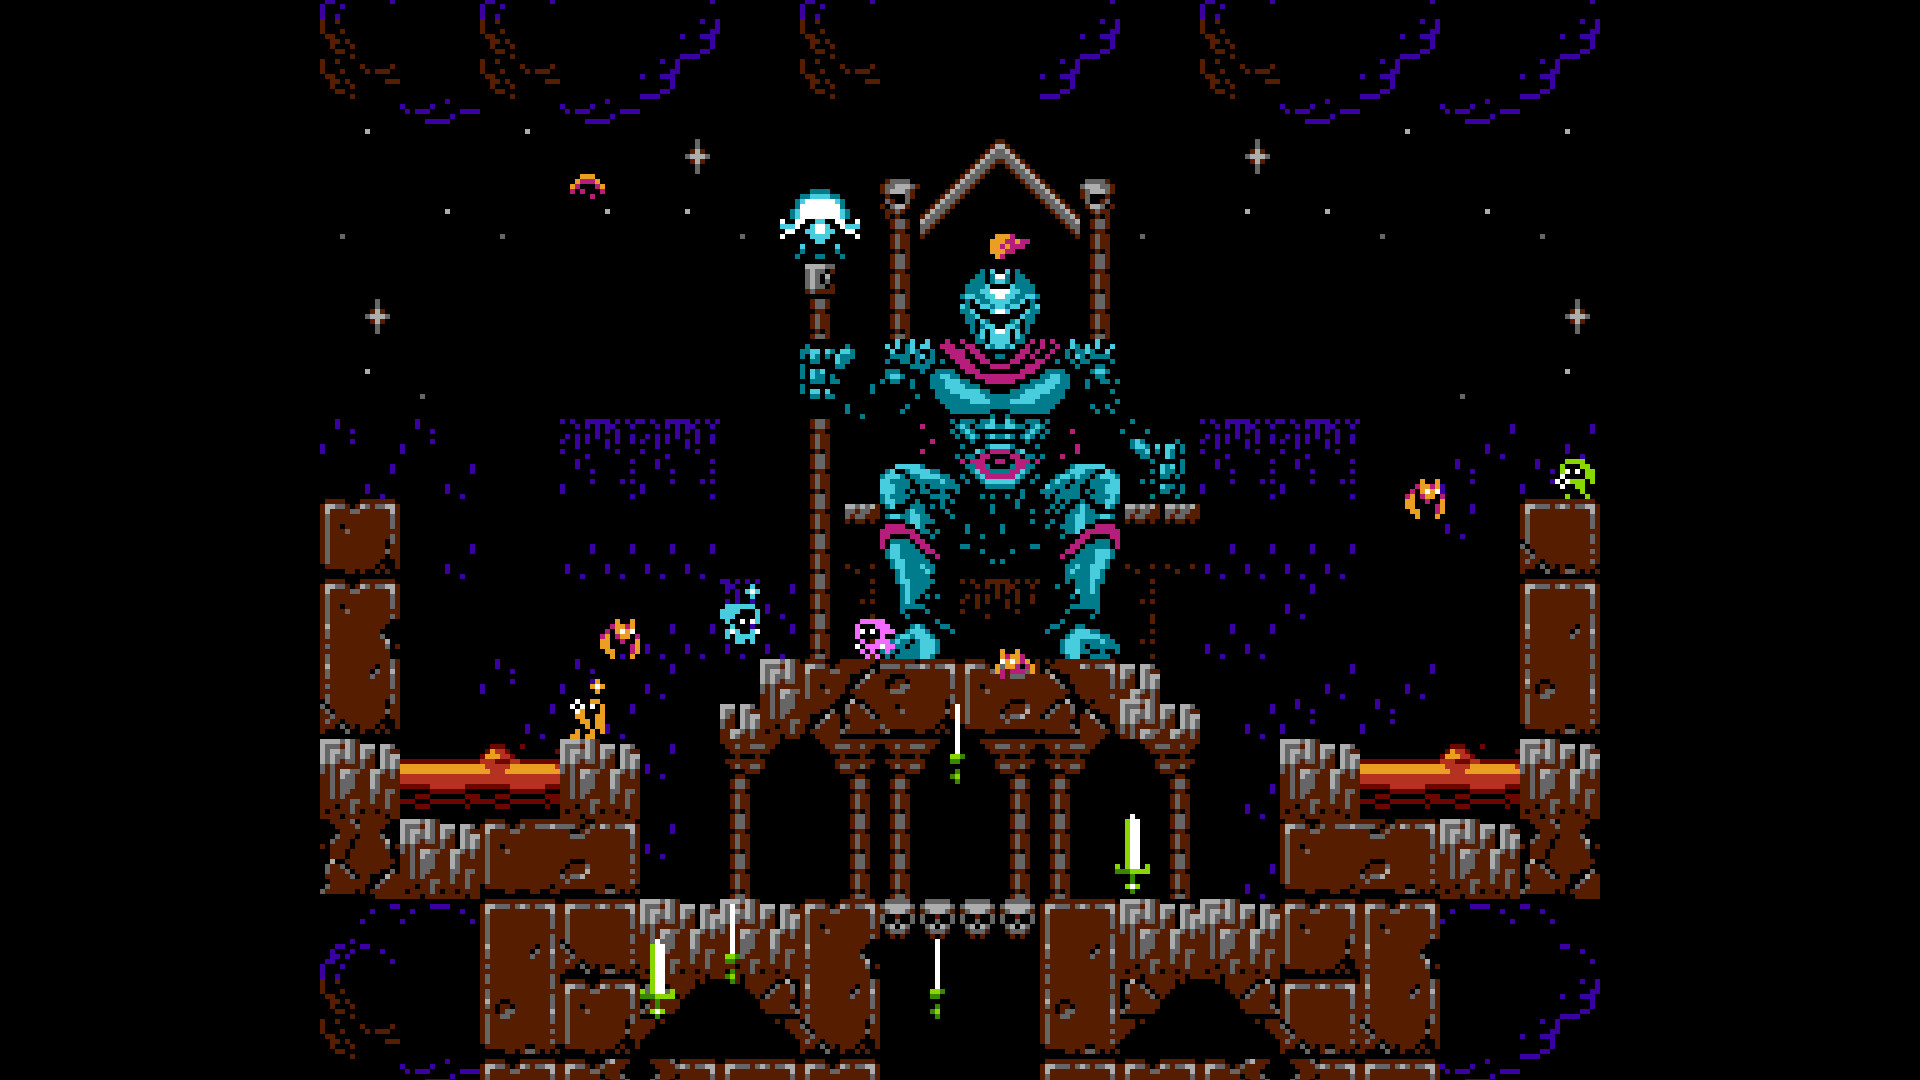
\includegraphics[width=1.0\textwidth]{Cuerpo/4/MM2.jpg} %
        \subcaption{Uno de los jefes del juego}
        \label{MM-Jefes}
    \end{minipage}
    \centering
    \begin{minipage}{0.43\textwidth}
        \centering
        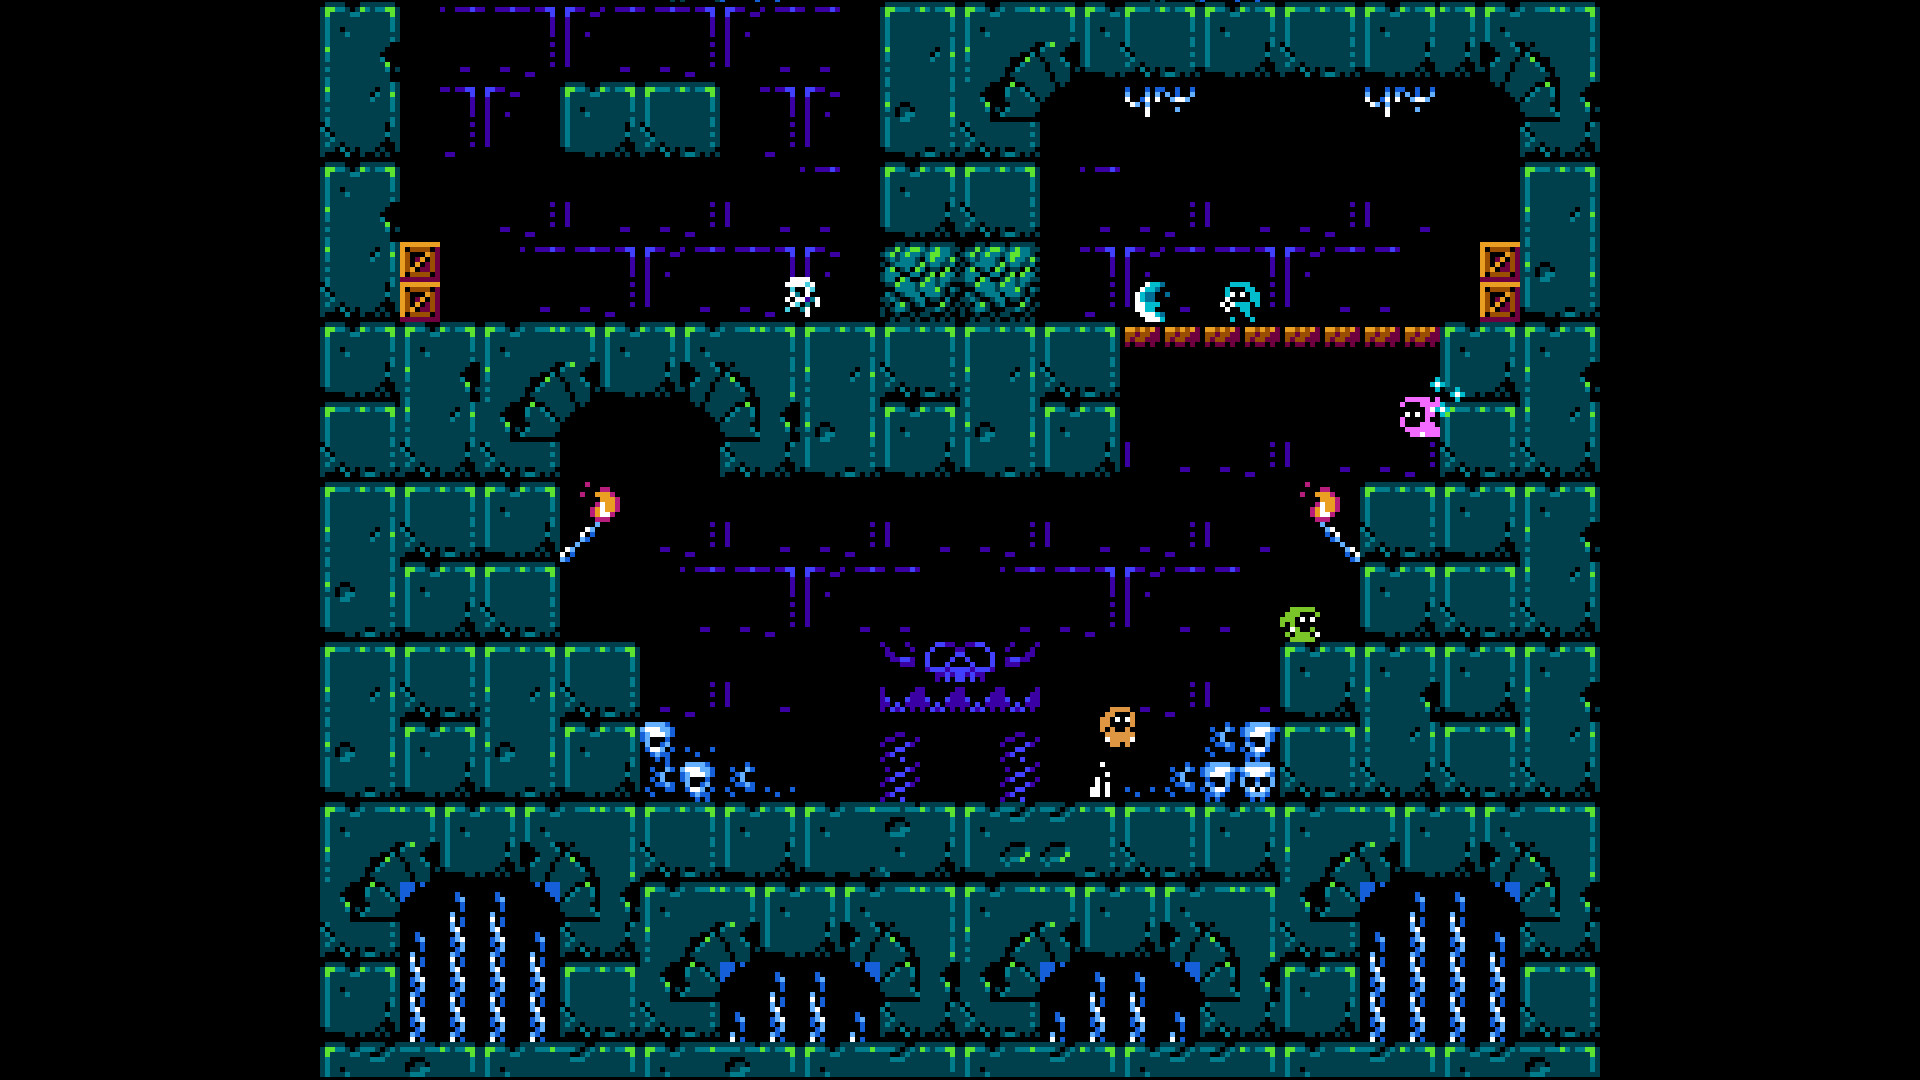
\includegraphics[width=1.0\textwidth]{Cuerpo/4/MM3.jpg} %
        \subcaption{Vario jugadores en un nivel}
        \label{MM-Jugadores}
    \end{minipage}
    \caption{Capturas de MicroMages}
\end{figure}

\textbf{Aspectos positivos}
\begin{itemize}
    \item Multijugador local para hasta 4 jugadores.
    \item Juego cooperativo.
    \item Distintos modos de dificultad.
    \item Juego de 40KB de memoria.
\end{itemize}

\textbf{Aspectos negativos}
\begin{itemize}
    \item El gameplay tiende a hacerse repetitivo.
    \item Difícil de visualizar los sprites si no se tiene buena vista.
    \item Niveles y enemigos repetitivos.
\end{itemize}

\subsubsection{Risk of Rain}

\emph{Risk of Rain}, desarrollado por \emph{Hopo Games} y publicado por
\emph{Gearbox Publishing} en el 2013, es un juego de acción y plataformas con
elementos roguelike (especificamente muerte permanente). Los jugadores deberán
intentar conseguir avanzar lo más que puedan batallando con seres hostiles para
escapar del planeta. A través de cada nivel podrán encontrar objetos aleatorios
que les ayudarán a progresar otorgándoles habilidades especiales. El juego está
disponible para PC, PS4, PS Vita, Nintendo Switch, Xbox One y su modelo de
negocio es Buy-to-Play.

La similitud que tiene el producto con este juego recae en el hecho de que ambos
son de \emph{plataformas} y de \emph{acción} con elementos \emph{roguelite}. En
efecto, éste ha sido una inspiración directa para la idea de usar múltiples
artefactos aleatorios y la de generar los niveles de manera procedural.

La página oficial es:
\url{https://riskofraingame.com/}

\textbf{Capturas}

\begin{figure}[H]
    \centering
    \begin{minipage}{0.43\textwidth}
        \centering
        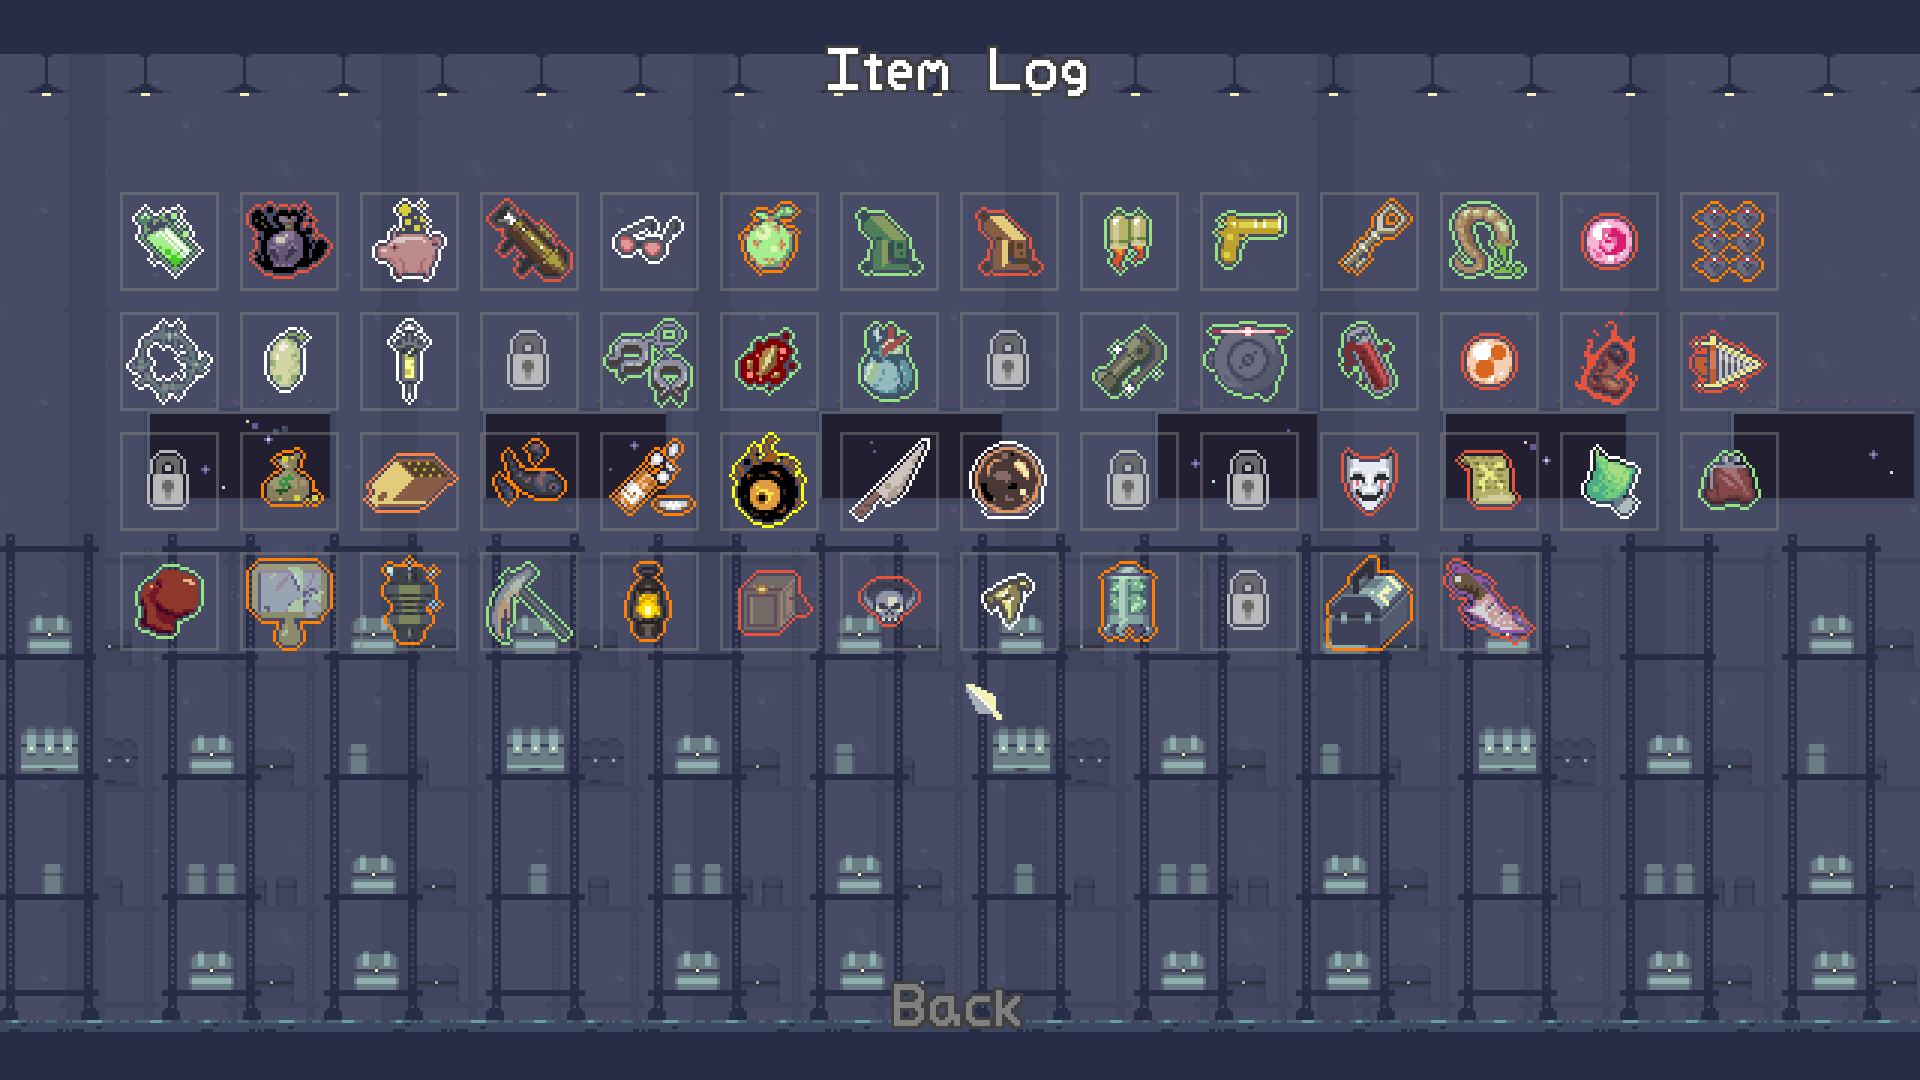
\includegraphics[width=1.0\textwidth]{Cuerpo/4/RoR1.png} %
        \subcaption{Menú de objetos encontrados}
        \label{RoR-Objetos}
    \end{minipage}\hfill
    \begin{minipage}{0.43\textwidth}
        \centering
        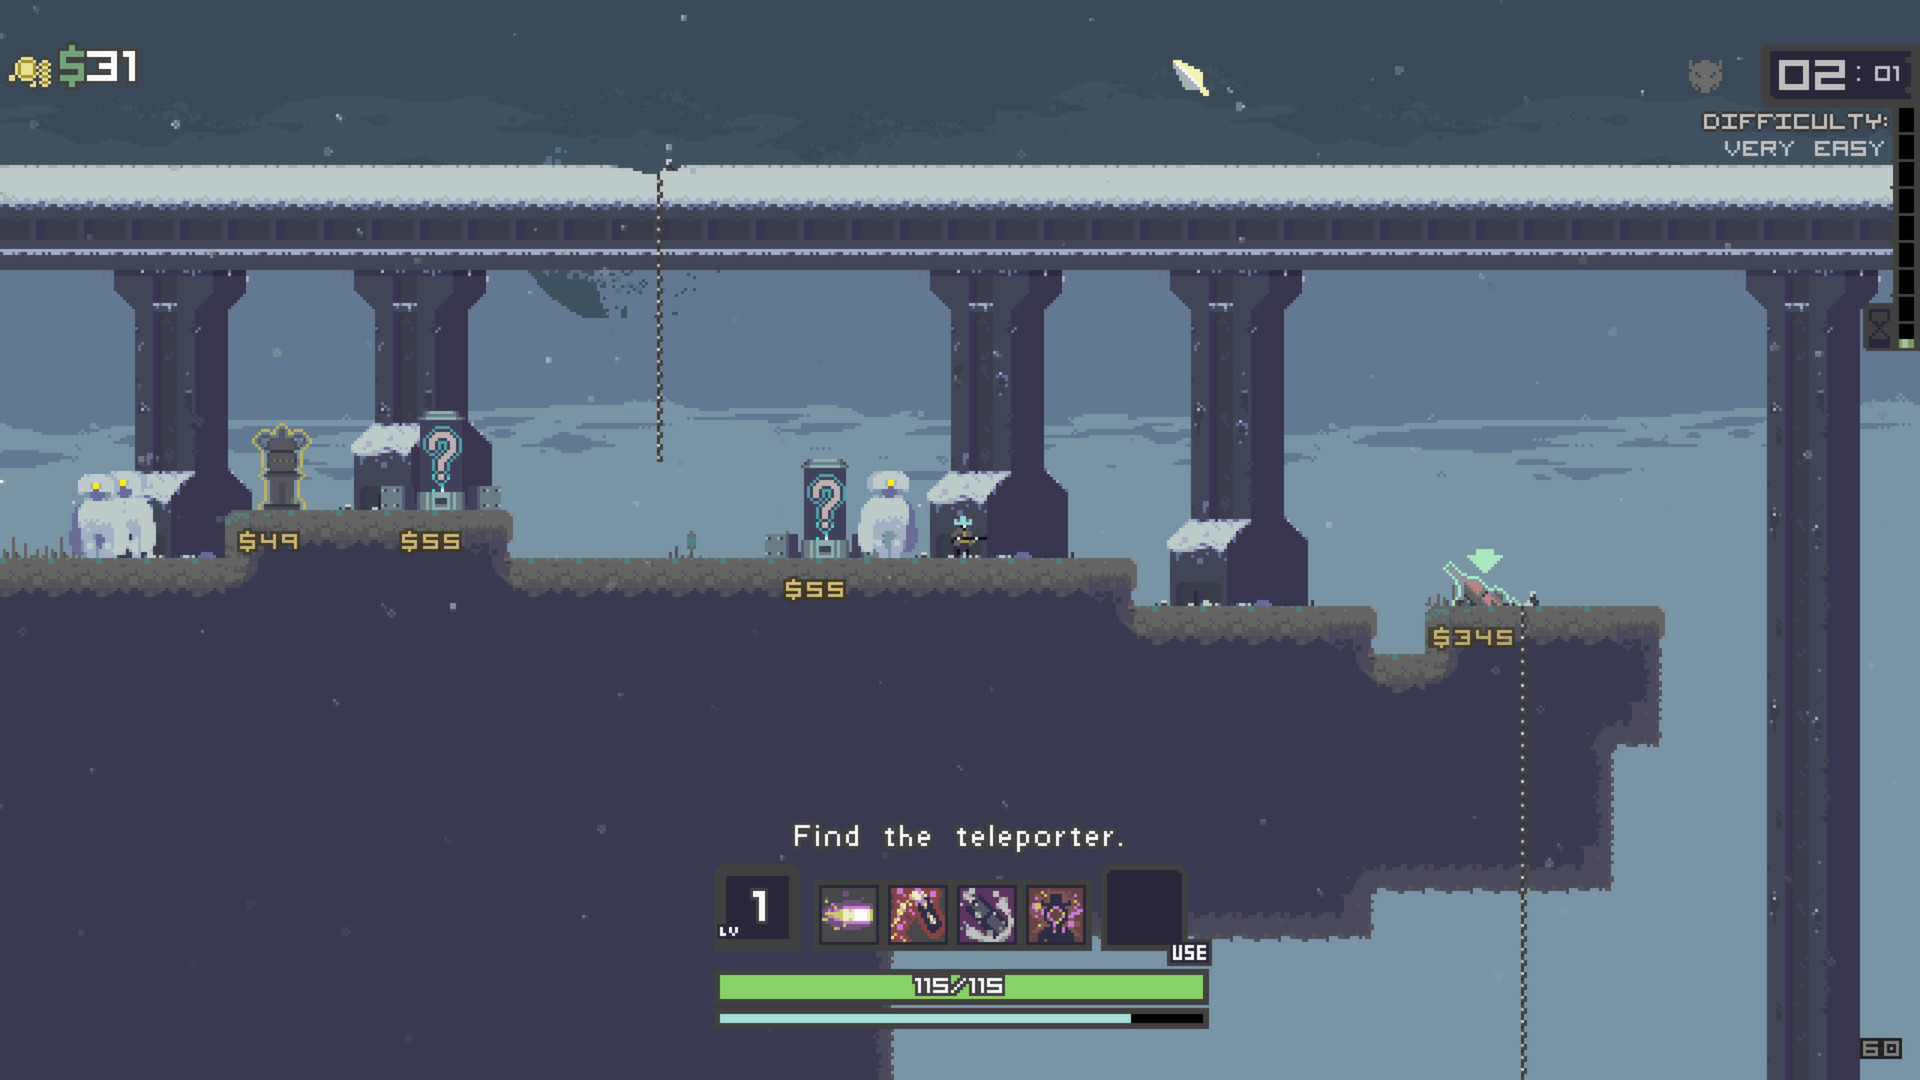
\includegraphics[width=1.0\textwidth]{Cuerpo/4/RoR2.jpg} %
        \subcaption{Un nivel del juego con enemigos}
        \label{RoR-Nivel}
    \end{minipage}
% \end{figure}
    \centering
% \begin{figure}[H]
    \begin{minipage}{0.43\textwidth}
        \centering
        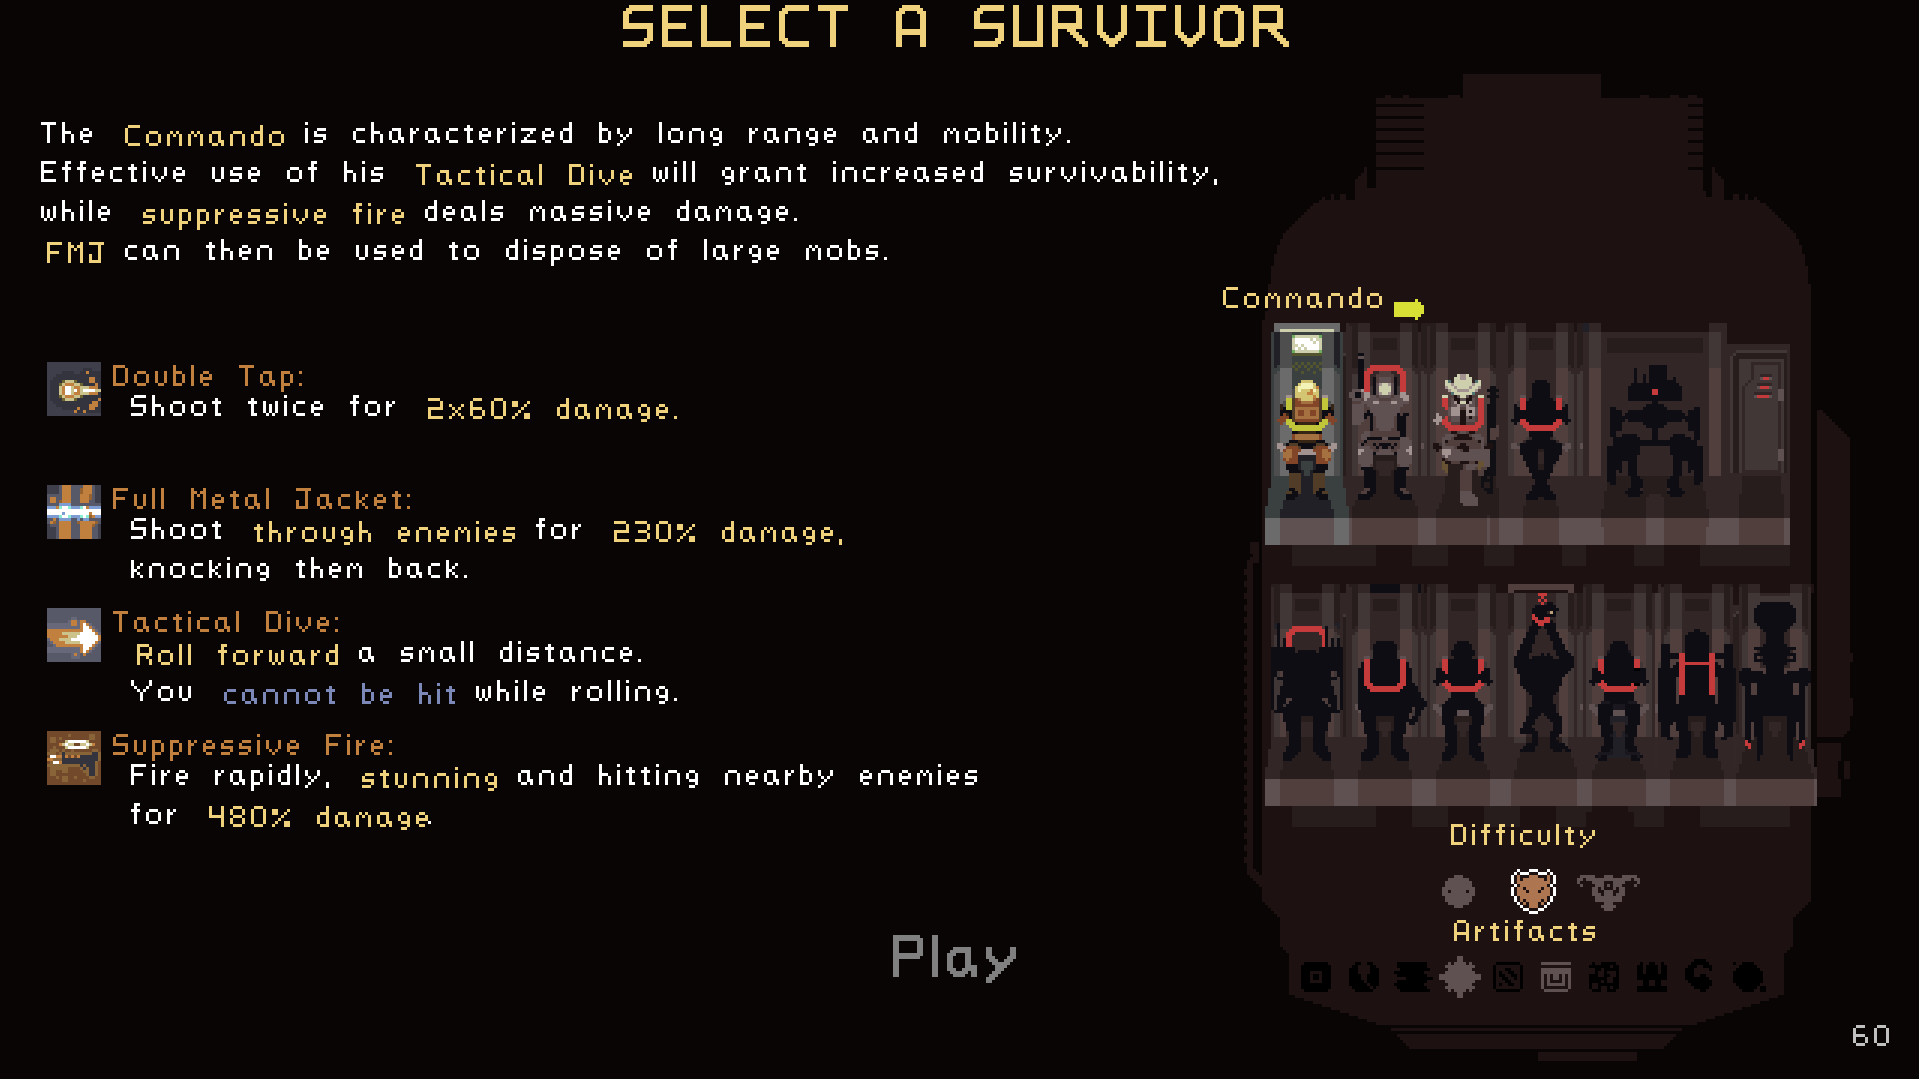
\includegraphics[width=1.0\textwidth]{Cuerpo/4/RoR3.jpg} %
        \subcaption{Menú de selección de personaje}
        \label{RoR-Personajes}
    \end{minipage}
    \caption{Capturas de Risk of Rain}
\end{figure}

\textbf{Aspectos positivos}
\begin{itemize}
    \item Multijugador local y online hasta 4 jugadores.
    \item Distintas clases para distintos estilos de juego.
    \item Una gran cantidad de coleccionables y secretos.
    \item Habilidades especiales que son capaces de cambiar la estrategia de juego.
\end{itemize}

\textbf{Aspectos negativos}
\begin{itemize}
    \item Muy difícil para el público casual.
    \item Las partidas pueden hacerse demasiado largas.
    \item El juego sufre de algunos problemas técnicos para usar las opciones de multijugador.
\end{itemize}